\documentclass{beamer}

\usefonttheme{serif}

\setbeamertemplate{footline}[frame number]{}
\setbeamertemplate{navigation symbols}{}

\usecolortheme{default}
\setbeamercolor{block title}{bg=lily!20,fg=black}
\setbeamercolor{block body}{bg = blue!10, fg = black}
\setbeamertemplate{itemize item}[square]
\setbeamercolor{itemize item}{fg = cyan}
\setbeamercolor{enumerate item}{fg = cyan}

\usepackage{multimedia}

\usetheme{default}

%\setbeamercolor{titlelike}{fg=black}
%Information to be included in the title page:
\title{Sample title}
\author{Anonymous}
\institute{Overleaf}
\date{2021}

\title[About Beamer] %optional
{Pockels effect}

%\subtitle{A short story}

\author[Arthur, Doe] % (optional, for multiple authors)
{D.~Dedkov }

\institute[VFU] % (optional)
{
	Moscow Institute of Physics and Technology
}

\date[VLC 2023] % (optional)
%{Very Large Conference, April 2021}

%\logo{\includegraphics[height=1cm]{overleaf-logo}}

\begin{document}
	
\frame{\titlepage}

\begin{frame}
	\frametitle{Abstract}
	TODO
Adjusting screw Scatter plate Analyzer Screen Laser
Oscilloscope EMF source Photodiode
$$r_0 \;\; r_1\;\; r_2\;\; ...r_m$$
\end{frame}

\begin{frame}
	\frametitle{Birefringence}
	%\vspace{-30pt}
	\footnotesize
	In materials refractive index can depend on the polarization and propagation direction of light.
	\begin{figure}
		\footnotesize
		\centering
		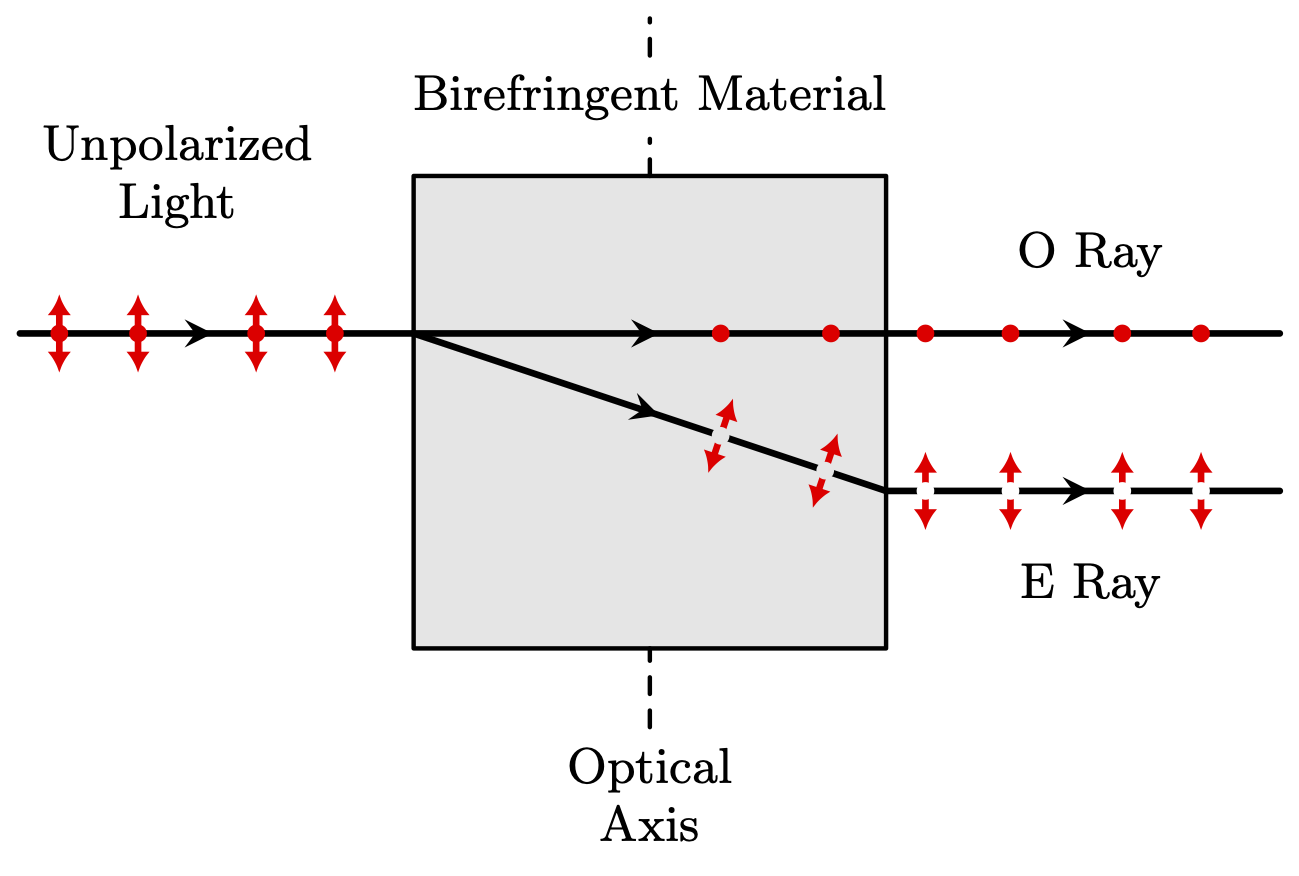
\includegraphics[width=0.8\linewidth]{res/birefringence}
		\vspace{-5pt}
		\footnotesize
		\caption{\footnotesize Ordinary ($n_o$) and extraordinary ($n_e$) waves scheme.}
	\end{figure}		
\end{frame}

\begin{frame}
	\frametitle{Analyzer}

	\begin{figure}
		\centering
		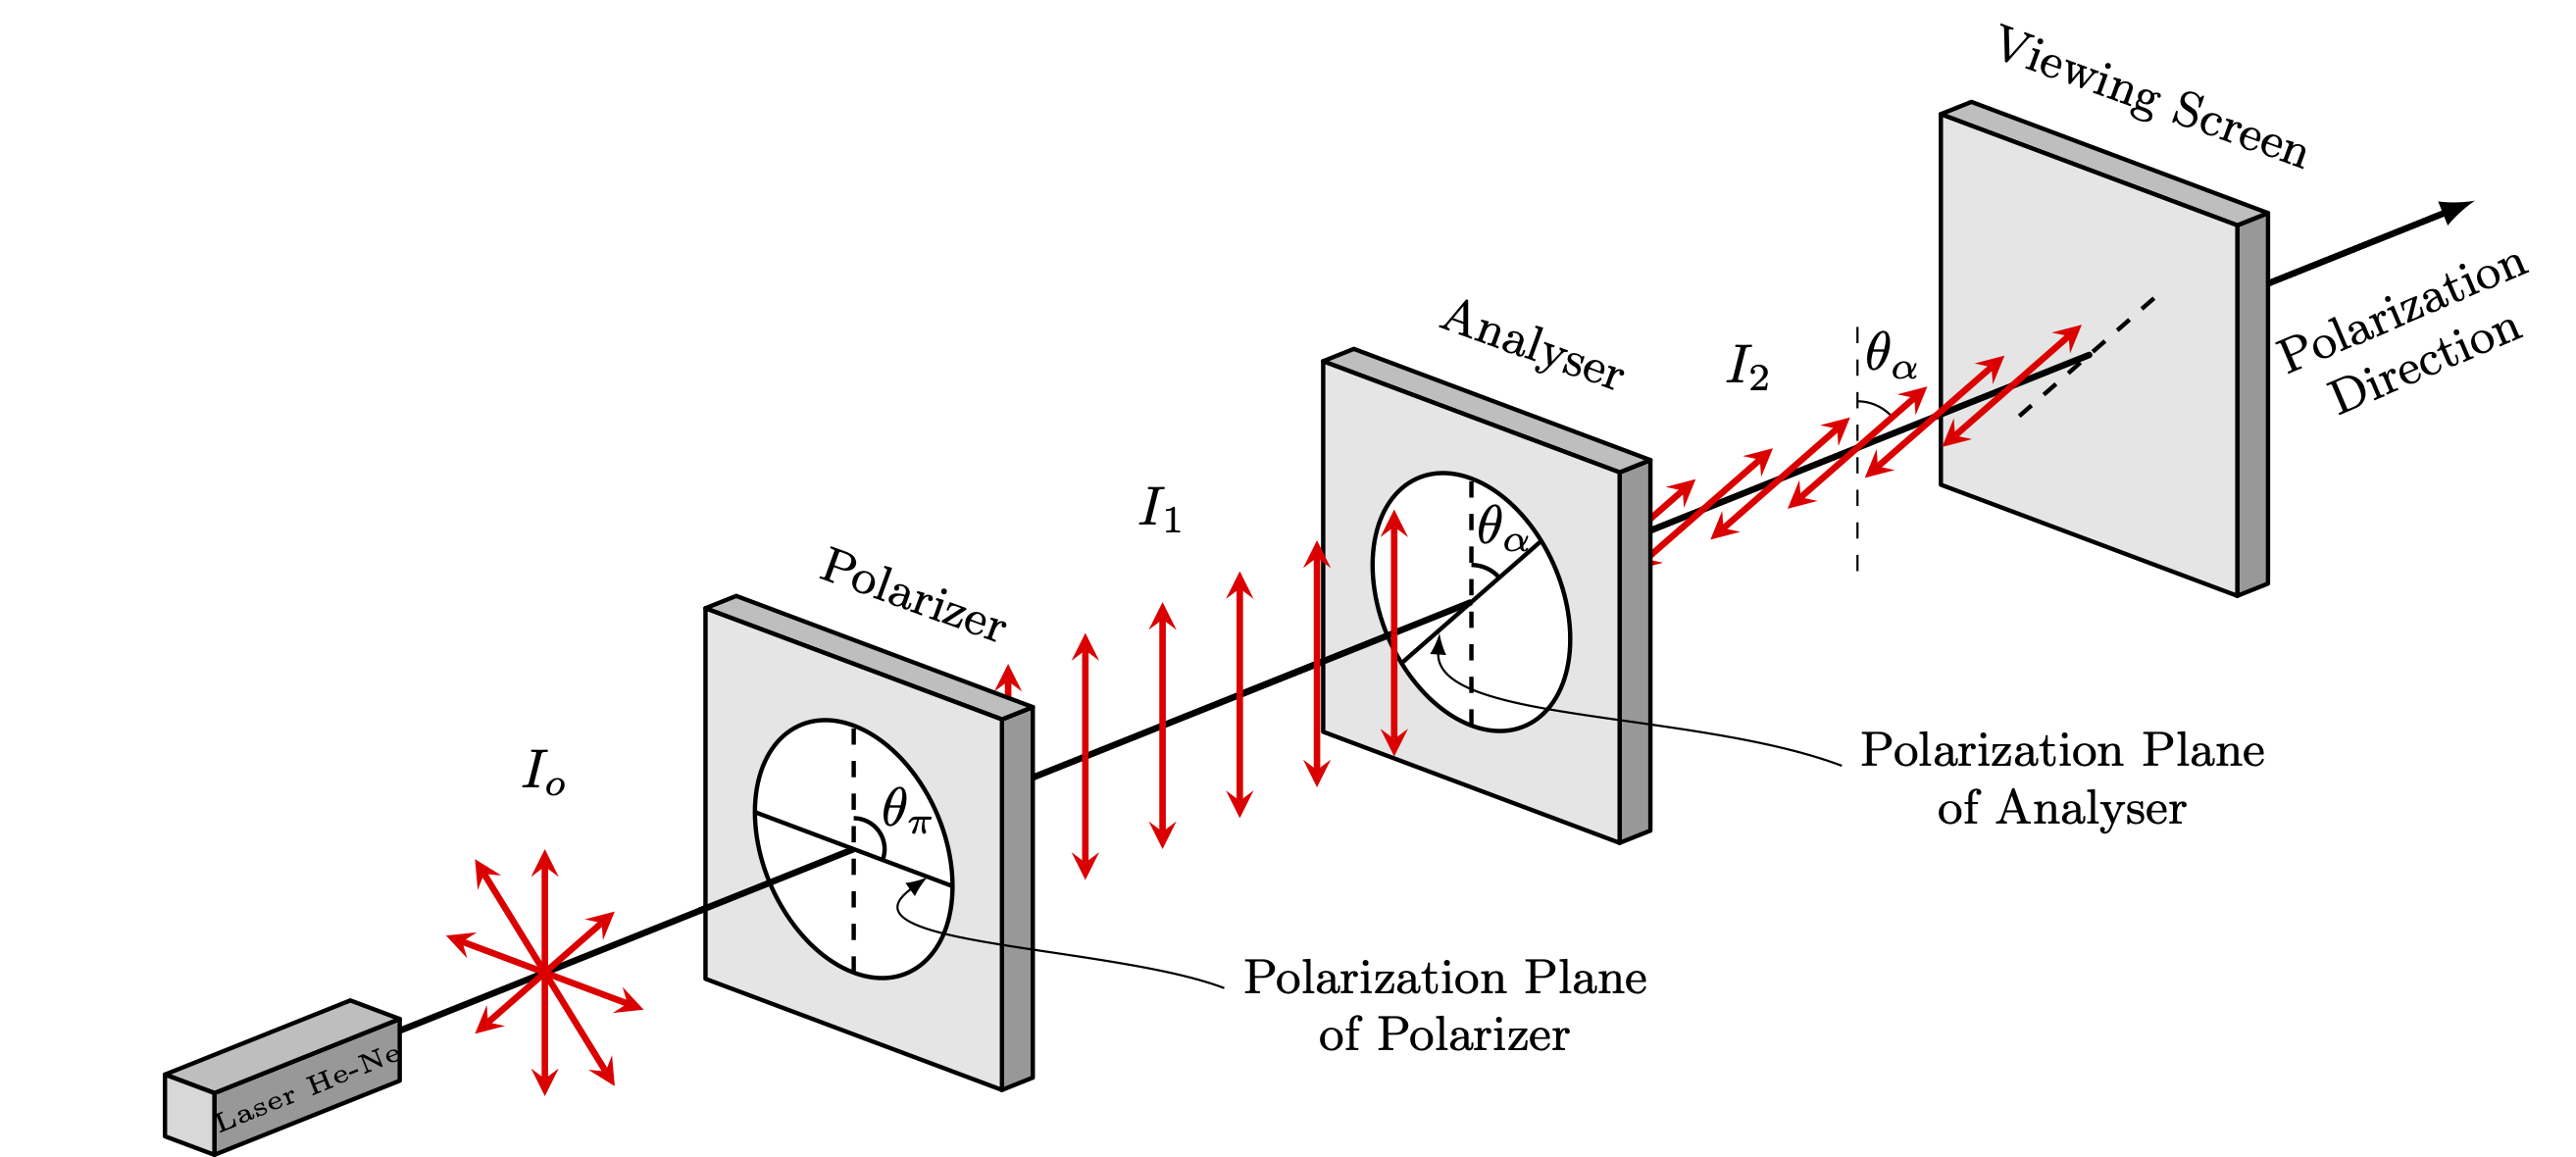
\includegraphics[width=1\linewidth]{res/polarizer_analyzer}
		\caption{Usage of analyzer}
	\end{figure}

	To describe polarization, analyzer and Malus' law is used:
	$$
	I(\theta_i) = I_0 \cos^2{\theta}.
	\label{eq:malus}
	$$
\end{frame}

	
\begin{frame}
	\frametitle{Scatter plate}		
	\begin{figure}
		\footnotesize
		\centering
		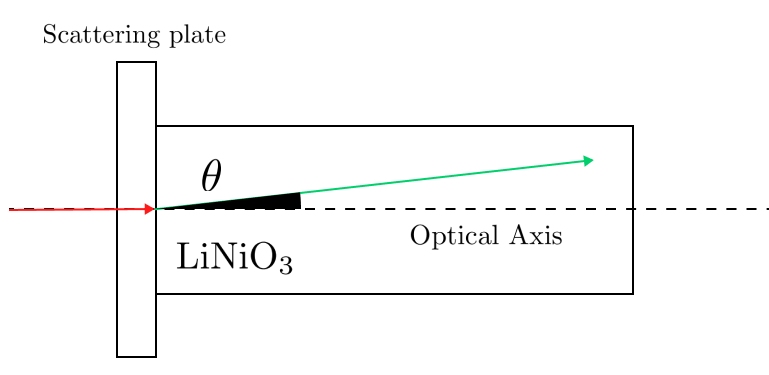
\includegraphics[width=0.9\linewidth]{res/theta_propagation}
		\vspace{-5pt}
		\footnotesize
		\caption{\footnotesize Ray propogation}
	\end{figure}
	
	\footnotesize
	\begin{itemize}
		\item[] \textbf{Ordinary}: Refractive index stays the same: $n_o(\theta) = n_o$
		
		\item[] \textbf{Extraordinary}: Refractive index can be assumed from:
		
		$$\frac{1}{n_e^2(\theta)} = \frac{\cos^2{\theta}}{n_o^2} + \frac{\sin^2{\theta}}{n_e^2} \implies n_e^2(\theta) \approx n_o - (n_o - n_e) \theta^2$$
	\end{itemize}	
\end{frame}

\begin{frame}
	\frametitle{Interference observation}
	
	\begin{figure}
		\centering
		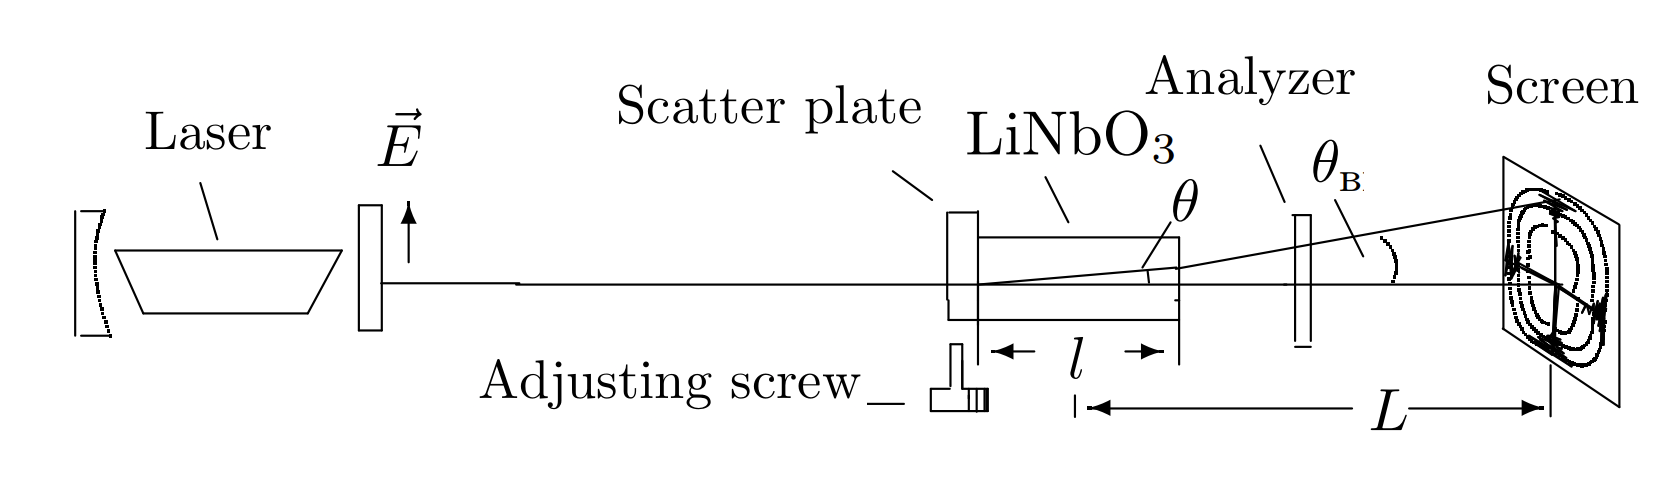
\includegraphics[width=1\linewidth]{res/scheme}
		\caption{Experimental setup}
	\end{figure}
	
	Phase shift between ordinary and extraordinary waves can be estimated:
	$$
	\Delta \varphi = \frac{2\pi}{\lambda}l(n_o - n_e)\theta^2,
	$$
	where $\lambda$ -- wavelength, $l$ -- LiNiO$_3$ crystal length.
\end{frame}

\begin{frame}
	\frametitle{Conoscopic interference patterns}
	
	\begin{figure}
		\centering
		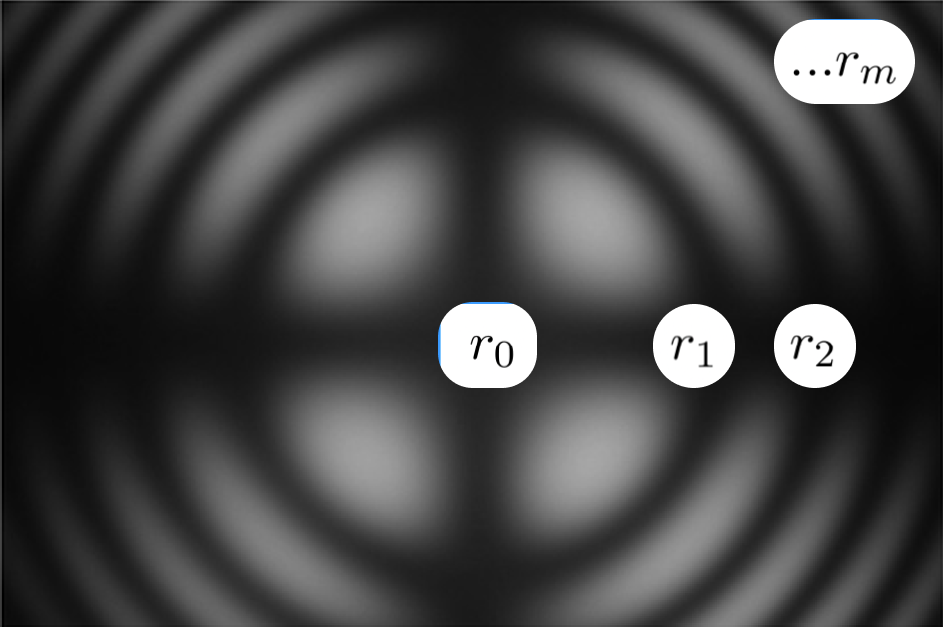
\includegraphics[width=0.5\linewidth]{res/pattern}
		\caption{Conoscopic interference pattern with the dark "maltese cross"}
	\end{figure}
	
	\footnotesize
	The radius of the nth ring can be calculated by equating: $\Delta \varphi = 2 \pi m$
	$$r^2_m = \frac{\lambda}{l} \frac{(n_o L)^2}{(n_o-n_e)} m,\;\; m = 1,2...,$$
	
	where $L$ -- distance from crystal to the screen.
\end{frame}
	
\begin{frame}[plain,c]	
	\begin{center}
		\huge \usebeamercolor[fg]{frametitle} Measurements and Results
	\end{center}
\end{frame}	

\begin{frame}
	\frametitle{Experimental setup}
	\begin{figure}
		\centering
		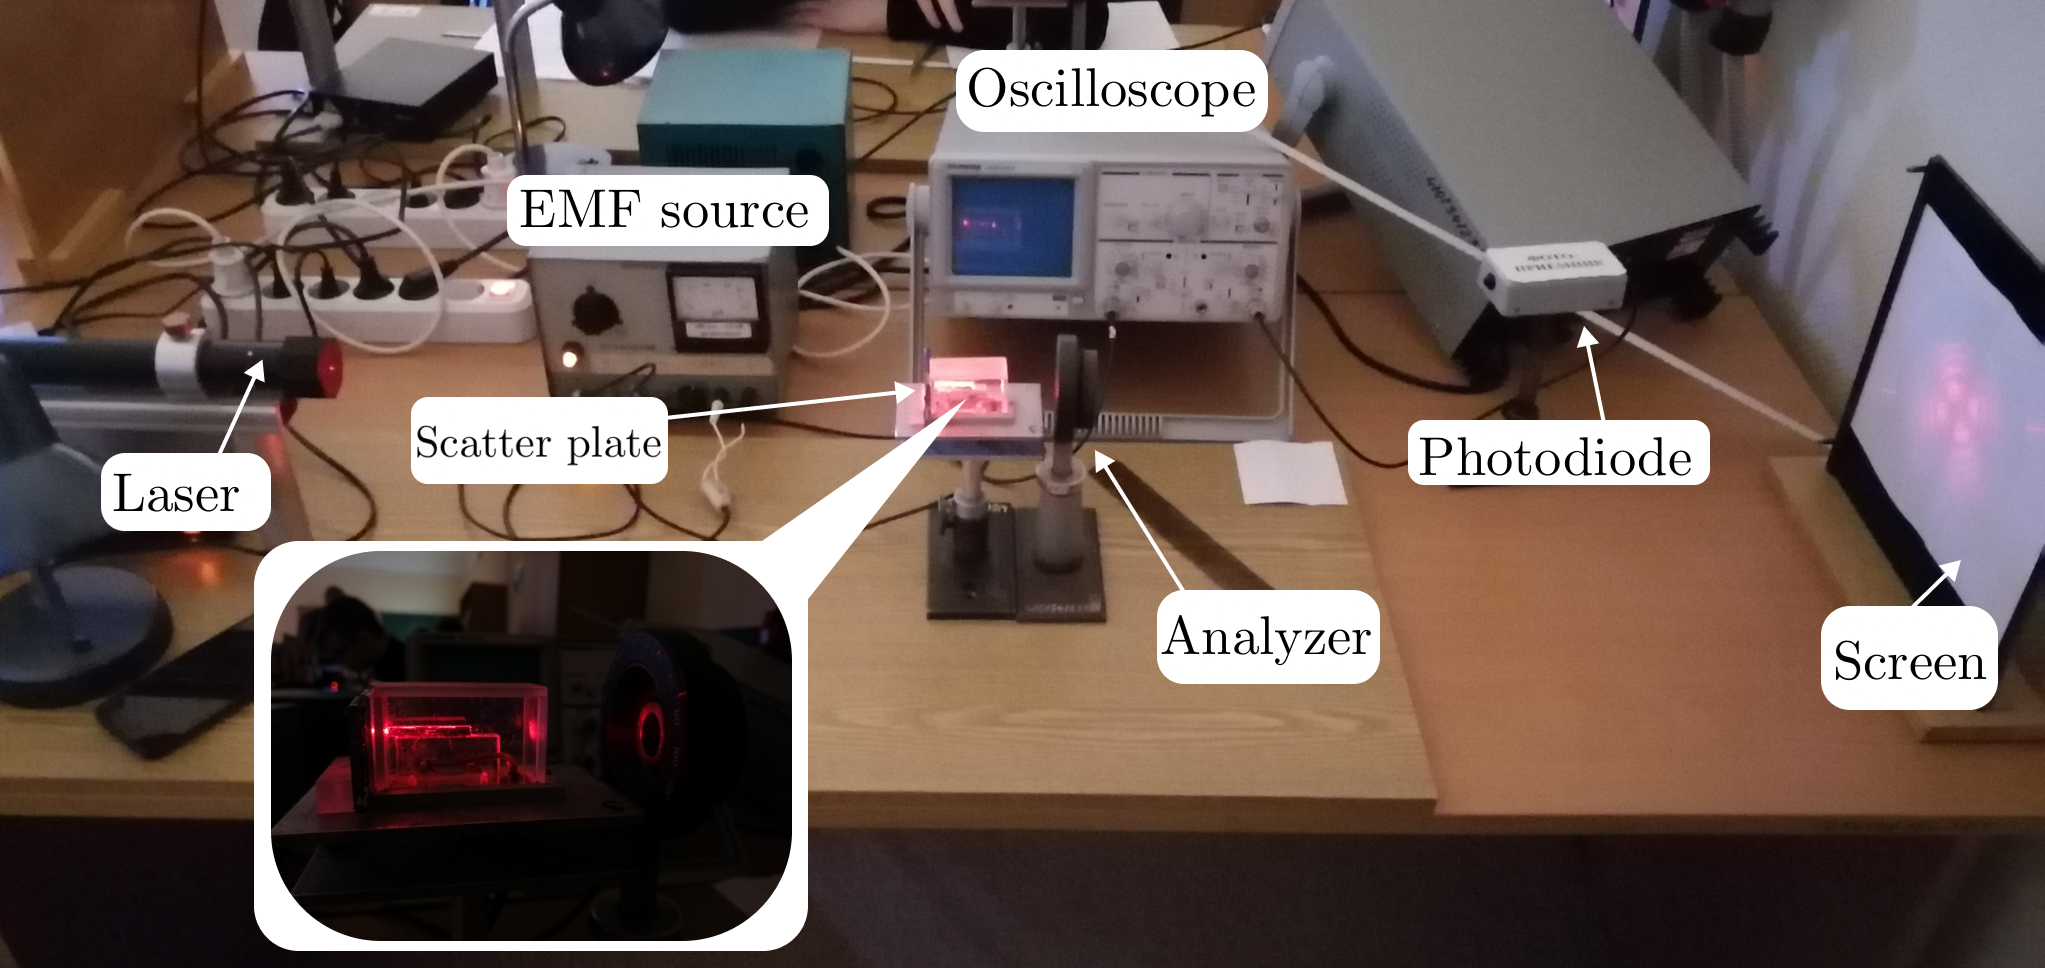
\includegraphics[width=1\linewidth]{res/setup}
		\vspace{-10pt}
		\caption{\footnotesize Photo of the experimental setup. }
	\end{figure}
\end{frame}

\begin{frame}
	\frametitle{Conoscopic interference patterns}
	\begin{figure}
		\centering
		\includegraphics[width=1\linewidth]{res/meltese_cross}
		\vspace{-10pt}
		\caption{\footnotesize  Dark (left) and light (right) "maltese cross" patterns. When the polarizer is rotated by 90 degrees, the cross pattern changes to a bright cross on a dark background. }
	\end{figure}
\end{frame}

\begin{frame}
	\frametitle{Dark rings}
	\begin{columns}
	\begin{column}{0.5\textwidth}
		\begin{figure}
			\centering
			\includegraphics[width=1\linewidth]{res/pattern_lines}
			\caption{\footnotesize Conoscopic interference patterns rings }
		\end{figure}
	\end{column}
	\begin{column}{0.5\textwidth}
		\begin{figure}
			\centering
			\includegraphics[width=1\linewidth]{gen/plot}
			\caption{\footnotesize Linearization $r_m^2(m)$}
		\end{figure}
	\end{column}
\end{columns}	
\footnotesize
From the series $r_m(m)$ we can calculate the birefringence difference using slope: 
$$\Delta n = n_o - n_e = \frac{\lambda}{l} \frac{(n_o L)^2}{\frac{\partial r^2_m}{\partial m}} = (0.098 \pm 0.004)$$

\end{frame}



\begin{frame}
	\frametitle{Half-wave voltage}
	
	\begin{figure}
		\centering
		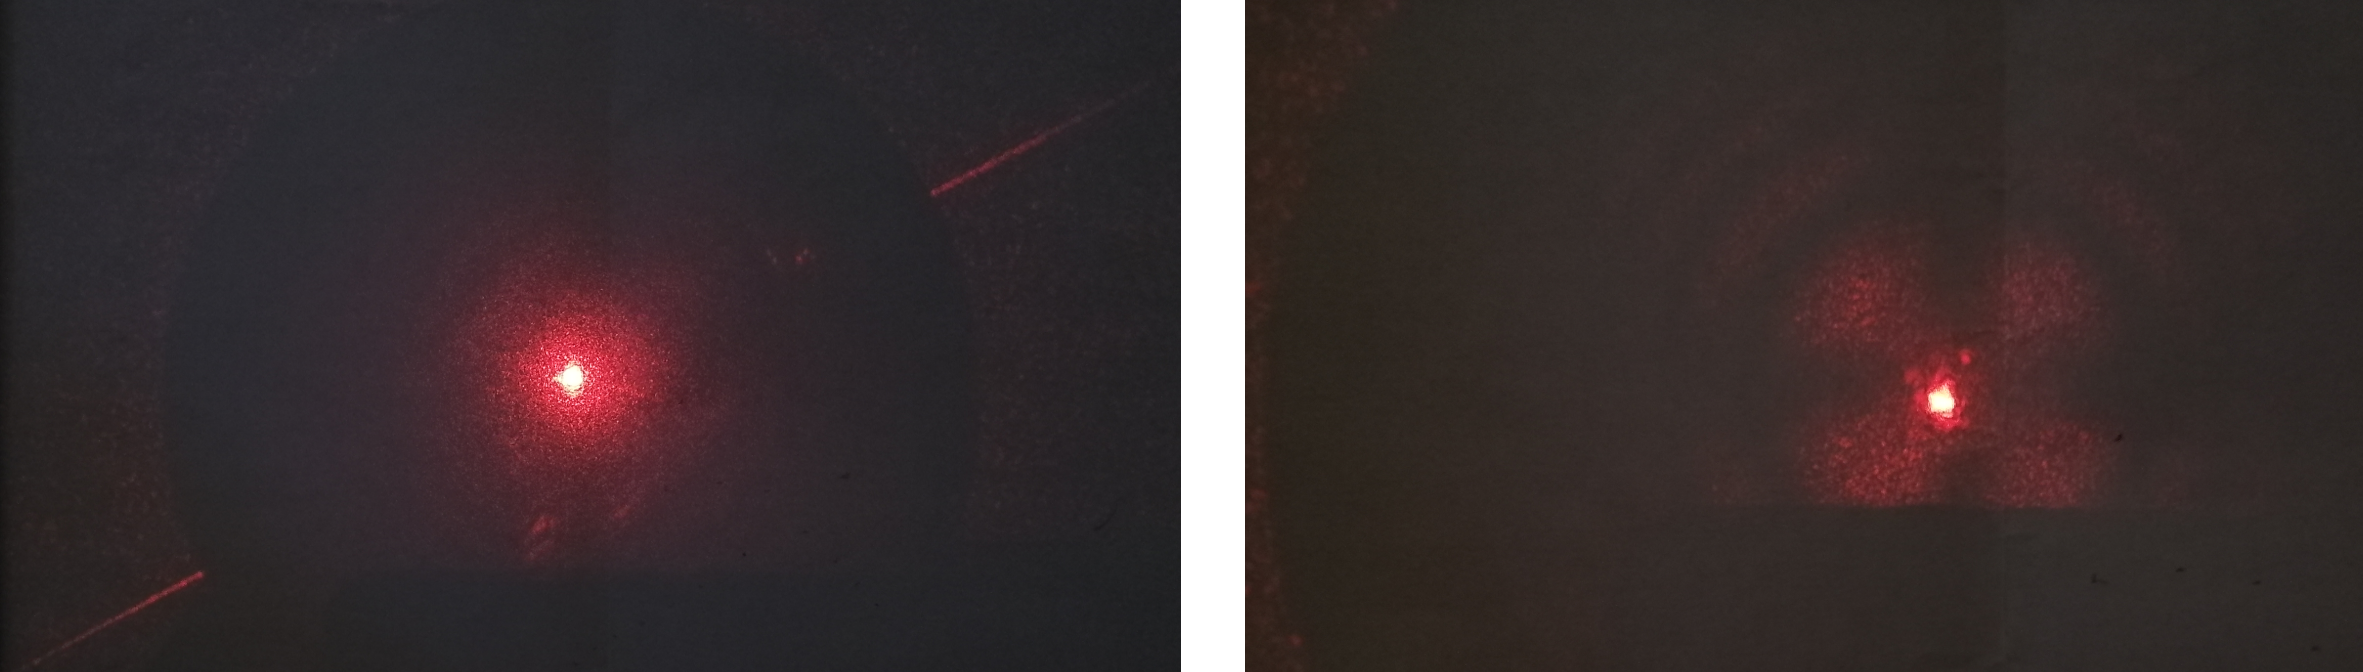
\includegraphics[width=1\linewidth]{res/pockels_min_max}
		\caption{\footnotesize Photo of the maximum (left) and minimum (right) spot brightness observed with a change in voltage $U$.}
	\end{figure}
\begin{columns}
	\begin{column}{0.5\textwidth}
\begin{tabular}{lcc}
	\hline
	$$ & \multicolumn{2}{c}{$U, \text{kV}$} \\
	$$ & $\uparrow\uparrow$ & $\leftarrow\uparrow$ \\
	\hline
	$U_{\lambda/2}$ & $0.45$ & $0.45$ \\
	$U_{\lambda}$ & $0.94$ & $0.93$ \\
	$U_{3\lambda/2}$ & $1.38$ & $1.35$ \\
	\hline
\end{tabular}
	\end{column}
	\begin{column}{0.5\textwidth}
		The error is determined both by the division value of the voltmeter and by the eye of the experimenter:
		$\sigma_U \approx 0.06 \; \text{kV}$
	\end{column}
\end{columns}	
\end{frame}


\begin{frame}
	\frametitle{Quarter-wave voltage}
	\begin{figure}
	\centering
	\movie[width=\linewidth, height=0.5625\linewidth, poster, borderwidth=1pt]{}{res/lambda_4.mp4}
    \end{figure}
\end{frame}
	
\begin{frame}
	\frametitle{Oscilloscope}
	\begin{figure}
		\centering
		\includegraphics[width=1\linewidth]{res/oscilloscope_parallel}
		\caption{\footnotesize Photo waveforms for parallel polarizations.}
	\end{figure}
	\begin{figure}
		\centering
		\includegraphics[width=1\linewidth]{res/oscilloscope_perpendicular}
		\caption{\footnotesize Photo waveforms for perpendicular polarizations.}
	\end{figure}
	
\end{frame}	
	
	
\begin{frame}
	\frametitle{Results}
	Investigated the interference of scattered light passing through the crystal.
	Determined birefringence difference:
	
	 $$\Delta n = (0.098 \pm 0.004) \; (\text{reference value}\;\; n_o - n_e = 0.10).$$
	
	 Observed the change in the nature of the polarization of light when an electric field was applied to a crystal. Estimated half-wave voltage:
	 $$U_{\lambda/2} = (0.45 \pm 0.06) \;\text{kV}$$
	
\end{frame}

	
\end{document}